%----------------------------------------------------------------------------------------
%	PREÁMBULO
%----------------------------------------------------------------------------------------


\documentclass[11pt, oneside]{book}
\usepackage[paperwidth=17cm, paperheight=22.5cm, bottom=2.5cm, right=2.5cm]{geometry}

% El borde inferior puede parecerles muy amplio a la vista. Les recomiendo hacer una prueba de impresión antes para ajustarlo

\usepackage{amssymb,amsmath,amsthm} % Símbolos matemáticos
\usepackage[spanish,mexico,es-tabla]{babel}
\usepackage[utf8]{inputenc} % Acentos y otros símbolos 
\usepackage{enumerate}
\usepackage{optidef}
\usepackage{hyperref} % Hipervínculos en el índice
\usepackage[spanish]{cleveref}
\usepackage{graphicx}
\usepackage[usenames,dvipsnames]{xcolor} % Color
%\usepackage{subfig} % Subfiguras
\usepackage{listings}%Para los códigos de MALTAB, ver documentación de matlab-prettifier
\usepackage[framed]{matlab-prettifier}
\usepackage[linesnumbered,lined,boxruled,spanish,onelanguage]{algorithm2e}
\usepackage{titling}
\usepackage{amsfonts}
\usepackage[thinc]{esdiff}
\spanishdecimal{.}
\definecolor{itamgreen}{RGB}{0,104,83}
\hypersetup{
    colorlinks=true,
    linkcolor=itamgreen,
    filecolor=itamgreen,      
    urlcolor=itamgreen,
    citecolor=itamgreen
}
\urlstyle{same}


\usepackage{translations}
\graphicspath{{Imagenes/}} % En qué carpeta están las imágenes

\DeclareTranslationFallback{rank}{rank}
\DeclareTranslation{english}{rank}{rank}
\DeclareTranslation{spanish}{rank}{rango}

\DeclareMathOperator{\rank}{\GetTranslation{rank}}


% Para eliminar guiones y justificar texto
\tolerance=1
\emergencystretch=\maxdimen
\hyphenpenalty=10000
\hbadness=10000

\linespread{1.25} % Asemeja el interlineado 1.5 de Word

\let\oldfootnote\footnote % Deja espacio entre el número del pie de página y el inicio del texto
\renewcommand\footnote[1]{%
\oldfootnote{\hspace{0.05mm}#1}}

\newcommand{\bigO}[1]{\ensuremath{\mathop{}\mathopen{}\mathcal{O}\mathopen{}\left(#1\right)}}

\newcommand\smallO[1]{
    \mathchoice
    {% mode \displaystyle
      \scriptstyle\mathcal{O}\left(#1\right)
    }
    {% mode \textstyle
      \scriptstyle\mathcal{O}\left(#1\right)
    }
    {% mode \scriptstyle
      \scriptscriptstyle\mathcal{O}\left(#1\right)
    }
    {% mode \scriptscriptstyle
      \scalebox{0.7}{$\scriptscriptstyle\mathcal{O}$}\left(#1\right)
    }
}
  

\renewcommand{\thefootnote} {\textcolor{Black}{\arabic{footnote}}} % Súperindice a color negro

\setlength{\footnotesep}{0.75\baselineskip} % Espaciado entre notas al pie

\usepackage{fnpos} % Footnotes al final de pág.

\usepackage[justification=centering, font=bf, labelsep=period, skip=5pt]{caption} % Centrar captions de tablas y ponerlas en negritas

\newcommand{\imagesource}[1]{{\footnotesize Fuente: #1}}

\usepackage{tabularx} % Big tables
\usepackage{adjustbox}
\usepackage{longtable}


\usepackage{float} % Float tables

\usepackage{pgfplots} % Gráficas
\pgfplotsset{compat=newest}
\pgfplotsset{width=7.5cm}
\pgfkeys{/pgf/number format/1000 sep={}}

\newtheorem{theorem}{Teorema}[chapter]
\newtheorem{corollary}{Corolario}[theorem]
\newtheorem{lemma}[theorem]{Lema}
\newtheorem{definition}{Definición}
\newtheorem{plain}{Proposición}
\newtheorem{remark}{Corolario}[plain]

\newcommand{\Tr}[1]{\operatorname{Tr}\left(#1\right)}
\newcommand{\diag}[1]{\operatorname{diag}\left(#1\right)}
\newcommand{\frNm}[1]{\left\|#1\right\|_{\mathrm{F}}}

\SetKwBlock{Loop}{Repetir}{fin}

\usepackage{afterpage}
\newcommand\myemptypage{
    \null
    \thispagestyle{empty}
    \newpage
    }
    
    
\usepackage{todonotes}
%HAY Q BORRAR ESTOS COMMANDS EVENTUALMENTE
\newcommand{\val}[1]{\todo[color=blue!20!white]{\textbf{Vale:} #1}}
\newcommand{\valinline}[1]{\todo[inline,color=blue!20!white]{\textbf{Vale:} #1}}

\usepackage{natbib}

\usepackage{tcolorbox}

\usepackage{dirtytalk}

\usepackage[cache=false]{minted}
\usemintedstyle{bw}

\usepackage{multirow}

\begin{document}

%----------------------------------------------------------------------------------------
%	PORTADA
%----------------------------------------------------------------------------------------



\title{Una tesis extendida ($\overline{\text{tesis}}$)} 
\author{Valeria Aurora Pérez Chávez}

\begin{titlepage}
\begin{center}

\textsc{\Large Instituto Tecnológico Autónomo de México}\\[2em]

%Figura
\begin{figure}[h]
\begin{center}

\includegraphics[scale=0.9]{logo-ITAM.pdf}
\end{center}
\end{figure}

% Pueden modificar el tamaño del logo cambiando la escala

\textbf{\LARGE \thetitle}\\[2em]

\textsc{\large Tesis}\\[1em]

\textsc{\large que para obtener el título de}\\[1em]

\textsc{\LARGE Licenciado en Matemáticas Aplicadas}\\[1em]

\textsc{\large Presenta}\\[1em]

\textsc{\LARGE \theauthor}\\[1em]

\textsc{\large Asesor: Ernesto Juvenal Barrios Zamudio}\\[1em]


% Asegúrense de escribir el nombre completo de su asesor con grado académico

\end{center}

\vspace*{\fill}
\textsc{Ciudad de México \hspace*{\fill} 2021} %El otro año es el bueno

\end{titlepage}



%----------------------------------------------------------------------------------------
%	DECLARACIÓN
%----------------------------------------------------------------------------------------

\thispagestyle{empty}

\vspace*{\fill}
\begingroup

\noindent
«Con fundamento en los artículos 21 y 27 de la Ley Federal del Derecho de Autor y como titular de los derechos moral y patrimonial de la obra titulada ``\textbf{\thetitle}'', otorgo de manera gratuita y permanente al Instituto Tecnológico Autónomo de México y a la Biblioteca Raúl Bailléres Jr., la autorización para que fijen la obra en cualquier medio, incluido el electrónico, y la divulguen entre sus usuarios, profesores, estudiantes o terceras personas, sin que pueda percibir por tal divulgación una contraprestación.»


\centering 

\vspace{3em}

\textsc{\theauthor}

\vspace{5em}

\rule[1em]{20em}{0.5pt} % Línea para la fecha

\textsc{Fecha}
 
\vspace{8em}

\rule[1em]{20em}{0.5pt} % Línea para la firma

\textsc{Firma}

\endgroup
\vspace*{\fill}

\newpage


%----------------------------------------------------------------------------------------
%	DEDICATORIA
%----------------------------------------------------------------------------------------

\thispagestyle{empty}
\pagenumbering{gobble}

\chapter*{Agradecimientos}

Agradezco a facu por ser tan chingona y a Mike por pasarme el formato. Salu2.
\begin{flushright}
\textsc{El Serch}
\end{flushright}
\newpage


\pagestyle{plain}
\frontmatter
%----------------------------------------------------------------------------------------
%	RESUMEN
%----------------------------------------------------------------------------------------
\include{Chapters/Resumen}


%----------------------------------------------------------------------------------------
%	ÍNDICE GENERAL
%---------------------------------------------------------------------------------------

\tableofcontents %Opcional pero sugerido, en especial si como Paco van a escribir un libro de 500 páginas. Es tesis, no enciclopedia.

%----------------------------------------------------------------------------------------
%	ÍNDICE DE CUADROS Y FIGURAS
%---------------------------------------------------------------------------------------

\listofalgorithms %Opcional
\newpage

\listoftables %Opcional

\listoffigures %Opcional

%----------------------------------------------------------------------------------------
%	TESIS
%----------------------------------------------------------------------------------------

\mainmatter % Empieza la numeración de las páginas

\pagestyle{plain}

% Incluye los capítulos en el fólder de capítulos

\chapter{Introducción}

\say{I always promote \textsf{Julia} among friends and colleagues in Latin America, even when it has been difficult to convince them because of the scarce resources of \textsf{Julia} in Spanish. I firmly believe in open access knowledge without barriers (either language barriers, accessibility, or others), and I will always advocate for that} \cite{articulo_10anos}. Las palabras de la chilena Pamela Bustamente, usuaria de \textsf{Julia},  engloban la razón de ser de esta tesis. 

Mi camino con \textsf{Julia} comenzó a principios del 2021 cuando tuve la oportunidad de trabajar en el Instituto Mexicano del Seguro Social (IMSS). \textsf{Julia} fue la herramienta que utilice para desarrollar un proyecto que estaba fundamentado en estadística bayesiana y requería de una gran cantidad de simulaciones. No tarde mucho tiempo en encontrarme con las dificultades que menciona Pamela y algunas más. Sin embargo, \textsf{Julia} debe tener otras cualidades que frecuentemente lo destaquen como un lenguaje prometedor que cada día va tomando más fuerza en la comunidad de programadores. 

Al principio, dichas cualidades eran un misterio para mí. Mi interrogante principal fue sobre la necesidad de crear este nuevo lenguaje. ¿Por qué usar \textsf{Julia} y no \textsf{Python} o \textsf{R}?, ¿Cuál fue la motivación de su creación? y, después de encontrarme con una falta de recursos, ¿Cómo es posible que 10 años más tarde hay tan poca ayuda de este lenguaje?  Esta tesis es mi esfuerzo por mostrar un nuevo lenguaje, sus alcances y hacer una comparativa con lo que ya se conoce. De paso, mi trabajo queda como evidencia y punto de partida para futuros usuarios hispanohablantes.  

Este trabajo no es un manual de \textsf{Julia} ni de ningún otro lenguaje. Eso ya existe. Lo que se busca es explicar pros y contras que se encontraron al utilizar \textsf{Julia}, \textsf{Python} y \textsf{R} en tres ejercicios distintos.

La tesis se divide en dos partes. El propósito de la primera parte es dar una imagen general de las funciones que se utilizaron en los tres lenguajes para crear la segunda parte. Primero, se expone la instalación de \textsf{Julia} en un sistema operativo \textsf{Windows} para después explicar aspectos básicos del lenguaje. También, se da una introducción a dos paquetes fundamentales para este trabajo. Esto se hace pensando que \textsf{Julia} es el lenguaje más reciente y se busca que el lector navegue fácilmente por el código presentado. Después, se presentan los paquetes y funciones que se utilizaron en \textsf{Python} y en \textsf{R} suponiendo que el lector ya está familiarizado con ellos. 

La segunda parte de la tesis consta de tres ejercicios cuyo objetivo es mostrar un aspecto diferente en los lenguajes. El primer ejercicio toma datos del National Institute of Standards and Technology (NIST) para medir la precisión numérica de cada lenguaje al hacer el ajuste de un polinomio de grado 10. El segundo ejercicio usa los datos del Censo de Población y Vivienda de México del 2020 hecho por el Instituto Nacional de Estadística y Geografía (INEGI). El objetivo de este ejercicio es el manejo y manipulación de una gran cantidad de datos. Finalmente, el tercer ejercicio presenta la programación de un algoritmo de búsqueda que se utiliza en la discriminación de modelos en diseños de experimentos. En este ejercicio, los cálculos son más intensivos por lo que busca medir la capacidad y velocidad de cómputo de los lenguajes. 

A continuación, se comienza este trabajo con la presentación de \textsf{Julia}. 




\chapter{Julia}

Julia es un lenguaje de programación gratis cuyo propósito general es ser tan rápido como C, pero manteniendo la facilidad de lenguaje de R o Python. Es una combinación de sintaxis simple con alto rendimiento computacional. Su slogan es "Julia se ve como Python, se siente como Lisp, corre como Fortran" \citep{Hackers}. 
Esta combinación de características hace que Julia sea un lenguaje de programación que ha tomado mucha fuerza en la comunidad científica. Ya que no es un lenguaje muy conocido, en esta sección explicaré como instalar Julia en una computadora con sistema Windows y algunos de los básicos del lenguaje.

\section{Reproducibilidad}
Antes de empezar, es necesario enfatizar que esta tesis es completamente reproducible. En Peng y Hicks definen que \say{un análisis de datos publicado es reproducible si el conjunto de datos y el código utilizados para crear el análisis de datos está disponible para que otros lo analicen y estudien de manera independiente} \cite{peng2021reproducible}. A pesar de que en el artículo enfatizan que esta definición puede ser un poco ambigua, sí resaltan que la reproducibilidad es un medio para revisar y, posteriomente, confiar en el análisis de otros. 

Por lo tanto, para este trabajo decidí publicar el código que utilicé en \textsf{GitHub}. Además, hago hincapié en las fuentes de los datos. A pesar de que esta tesis no es un manual de Julia, Python o R considero da suma importancia publicar mi trabajo para que les sirva a mis compañeros como referencia o punto de partida. 


\section{Instalación}
Este trabajo está hecho y escrito en Windows, por lo que explicaré la instalación de Julia y todas las demás aplicaciones en este sistema operativo. Sin embargo, sé que la instalación en Mac y Linux es muy similar y usualmente las instrucciones a seguir vienen en las mismas páginas que Windows. 

Al momento de la escritura y publicación de esta tesis la versión de Julia disponible es la \textbf{v1.6.3}. El primer paso ara descargar Julia, es entrar al link \url{https://julialang.org/downloads/}. 


En esta versión de Julia, las opciones disponibles de descarga son un instalador de 64-bits o uno de 32-bits. Para saber el tipo de Sistema que tiene tu ordenador debes seleccionar el botón de \textsf{Start}, después \textsf{Configuración} $>$ \textsf{Sistema} $>$ \textsf{Acerca de}. En esta opción puedes ver el tipo de sistema que tiene tu computadora. Con esta información, puedes elegir el instalador para tu computadora. Es importante seleccionar el \textsf{installer} y no el \textsf{portable}. Una vez descargado, seleccionas el archivo \textsf{.exe} y sigues los pasos de instalación. 

\section{Símbolo del sistema}
Una vez instalado puedes correr Julia desde el símbolo de sistema o desde otro programa como Atom, Visual Studio Code o Jupyter Notebook. Una de las ventajas de utilizar Julia desde el símbolo de sistema (también conocido como \textit{Command Prompt} o cmd) es que puedes controlar algunos parámetros del lenguaje. Mi sugerencia es que comiences a usar Julia directo desde el ícono que se genera automáticamente en la descarga. Después, cuando entiendas lo básico y empieces a generar programas que requieran mayor nivel computacional comiences a utilizar el cmd para correr Julia. Para facilitar esto, te recomiendo agregar Julia a un \textbf{PATH}. Las instrucciones para hacerlo en Windows 10 están en la página \url{https://julialang.org/downloads/platform/#windows}.

\subsection{\textit{Multithreading}}
Una de las razones por la que Julia tiene más velocidad que otros lenguajes es porque  tiene la capacidad para multihilo (\textit{multithreading} en inglés). Esto significa que puede correr diferentes tareas de manera simultánea en varios hilos. Explicado de la manera más simple, la meta de los autores de Julia fue hacer un lenguaje de programación con un rendimiento tan alto que pudiera hacer varias cosas a la vez. Debido a que uno de los objetivos de esta tesis es medir la eficiencia y velocidad de Julia, es crucial conocer la característica del \textit{multithreading} y como utilizarla. 

Si estás usando Julia por medio del cmd es necesario modificar la cantidad de hilos que se van a utilizar antes de ejecutar Julia.  En Windows, esto se hace escribiendo \texttt{set JULIA\_ NUM\_ THREADS=4} \citep{manual_Julia}. Si estás trabajando con otro sistema operativo, este link te puede ayudar a cambiar la cantidad de hilos \url{https://docs.julialang.org/en/v1/manual/multi-threading/}. En este ejemplo, se cambiaron los hilos a 4, pero se puede poner cualquier número. Sin embargo, se recomienda que el número no exceda de la cantidad de procesadores físicos de la computadora. Después de hacer esta modificación, ahora sí podemos ejecutar Julia. 
  
Para observar que el cambio se ejecutó de manera correcta (en cualquiera de las dos opciones) basta con correr el comando \texttt{Threads.nthreads()} y observar que la respuesta sea el número deseado. 

\section{Básicos de Julia}
Como ya se mencionó, Julia busca ser un lenguaje de programación sencillo e intuitivo. Por lo tanto, su sintaxis es bastante sencilla. La asignación de variables se hace con un signo de igualdad $=$. El ejemplo más sencillo de esto sería \texttt{x = 2} donde denotamos a x el valor de 2. Toda la información sobre la sintaxis que utiliza Julia la obtuve del manual oficial de Julia \citep{manual_Julia}.

\subsection{Operaciones básicas}
La tabla \ref{operaciones_basicas_Julia} muestra la sintaxis usada para las operaciones básicas en Julia. 


\begin{center}
	\begin{tabular}{|c|c|c|} 
		\hline
		Expresión & Nombre & Descripción \\ 
		\hline 
		\texttt{+x} & suma unaria & la operación identidad \\ 

		\texttt{-x} & resta unaria & asigna a los valores sus inversos aditivos \\ 

		\texttt{x + y} & suma binaria & realiza adición \\ 

		\texttt{x - y} & resta binaria & realiza sustracción \\

		\texttt{x * y} & multiplicación & realiza multiplicación \\

		\texttt{x / y} & división & realiza divisiones \\

		\texttt{x $\div$ y} & división de enteros & $x / y$ truncado a un entero \\

		\texttt{x $\setminus$ y} & división inversa & equivalente a dividir \texttt{y / x} \\

		\texttt{x $\wedge$ y} & potencia & eleva \texttt{x} a la potencia \texttt{y} \\

		\texttt{x \% y} & residuo & equivalente a \texttt{rem(x,y)} \\
		
		\texttt{!x} & negación & realiza lo contrario de \texttt{x} \\
		
		\texttt{x \& \& y} & \textit{and} lógico & verifica si \texttt{x} y \texttt{y} se cumplen \\
		
		\texttt{x || y} & \textit{or} lógico & verifica si al menos uno, \texttt{x} o \texttt{y},  se cumplen \\
		\hline
	\end{tabular} 
	\captionof{table}{Operaciones básicas en Julia} \label{operaciones_basicas_Julia}
\end{center}


\subsubsection{Operaciones básicas en vectores}
En Julia, para cada operación binaria existe su correspondiente operación punto (\textit{dot operation} en inglés). Estas funciones están definidas para efectuarse elemento por elemento en vectores y matrices. Para llamarse, basta agregar un punto antes del operador binario. Por ejemplo,
 \texttt{[1 9 9 7] .$\wedge$ 2} eleva cada uno de los elementos del vector al cuadrado. 

También es importante mencionar que Julia maneja los números imaginarios utilizando el sufijo \texttt{im}. Sin embargo, no los utilice en este trabajo omitiré dar una mayor explicación. 

\subsection{\textit{Strings} (secuencias de caracteres)} 

Además de números, Julia puede asignar characteres a variables. Esto se hace utilizando las comillas dobles. Similar a otros lenguajes de programación, podemos accesar a caracteres específicos de un string utilizando corchetes cuadrados $[$ $]$ y a cadenas seguidas de caracteres usando dos puntos $:$. Por ejemplo,

\begin{minted}{julia}
    julia> string = "Esta tesis es genial"
    julia> string[6]
    't': ASCII/Unicode U+0074 (category Ll: Letter, lowercase)
    
    julia> string[4:8]
    "a tes"
\end{minted}


Además, Julia también cuenta con la opción de concatenación de múltiples strings. Esto se hace utilizando un asterisco $*$ para separar cada uno de los strings. Por ejemplo,

\begin{minted}{julia}
	julia> grado = "licenciada"
	julia> nexo = "en"
	julia> carrera = "matematicas aplicadas"
	julia> espacio = " "
	julia> grado*espacio*nexo*espacio*carrera
	"licencia en matematicas aplicadas"
\end{minted}

\subsection{Funciones}
En Julia, una función es un objeto que asigna una tupla de argumentos a un valor de retorno \citep{Julia_manual}. La sintáxis básica para definir funciones en Julia es 

\begin{minted}{julia}
	function f(x, y)
		x + y
	end
\end{minted}

Además, puedes agregar la palabra \textit{return} para que la función regrese un valor. Por ejemplo, si quisieramos tener una función a la que le des dos números y te regrese el número mayor, la función sería la siguiente:

\begin{minted}{julia}
	function numero_mayor(x, y)
		if (x > y)
			return x
		else
			return y
		end
	end
\end{minted}


Para llamar a la función bastaría con escribir \texttt{numero\_mayor(x, y)} asignando o sustituyendo valores por $x$ y $y$. 

\subsection{Vectores y Matrices}

\begin{definition}
Un vector columna de $n$ componentes se define como un conjunto ordenado de $n$ números escritos de la siguiente manera:
\begin{equation*}
    \begin{aligned}
    \begin{pmatrix}
    x_1 \\ 
    x_2 \\
    \vdots \\
    x_n
    \end{pmatrix} 
    \end{aligned}
\end{equation*}
\end{definition}


En Julia, para definir un vector columna se hace uso de los corchetes cuadrados $[$ $]$ y comas. Por ejemplo, 

\begin{minted}{julia}
	julia> A = [1, 9, 9, 7]
	4-element Vector{Int64}
	1
	9
	9
	7
\end{minted}

da como resultado un vector de 4 elementos de tipo Int64. Es muy importante aprender a identificar como Julia lee los objetos ya que cada objeto tiene características y funciones diferentes.  

Si quisiera definir un vector renglón, se hace exactamente igual solamente omitiendo el uso de las comas. Sin embargo, es importante señalar que  ahora Julia tomó el objeto A como una matriz, no como un vector. 

\begin{definition}
Una matriz $A$ de $m \times n$ es un arreglo rectangular de $mn$ números dispuestos en $m$ renglones y $n$ columnas. 

\begin{equation*}
    \begin{aligned}
    \begin{pmatrix}
    a_{11} & a_{12} & \dots & a_{1j} & \dots & a_{1n} \\
    a_{21} & a_{22} & \dots & a_{2j} & \dots & a_{2n} \\
    \vdots &  \vdots  &  \ddots &  \vdots  & \ddots &\vdots\\
    a_{i1} & a_{i2} & \dots & a_{ij} & \dots & a_{in} \\
    \vdots &  \vdots  &  \ddots &  \vdots  & \ddots &\vdots\\
     a_{m1} & a_{m2} & \dots & a_{mj} & \dots & a_{mn} \\
    \end{pmatrix} 
    \end{aligned}
\end{equation*}
\end{definition}


En Julia, hay dos formas de definir matrices. La primera es utilizando los corchetes cuadrados $[$ $]$ para comenzar y terminar la matriz. Las columnas están separadas por espacios y las filas por punto y coma. La segunda opción similar a la primera con la única diferencia de que en lugar de punto y coma se cambia de renglón. Esta opción puede ser un poco tediosa ya que requieren que las columnas estén alineadas. Sin embargo, es una forma más visual de ver las matrices. En la siguiente tabla se pueden ver ambas opciones. 

\begin{minted}{julia}
	julia> A_1 = [1 2 3; 4 5 6]
	2x3 Matrix{Int64}
	1 2 3
	4 5 6
	julia> A_2 = [1 2 3
				4 5 6]
	2x3 Matrix{Int64}
	1 2 3
	4 5 6

\end{minted}

De manera análoga con los vectores, para llamar un solo elemento de la matriz se utilizan los corchetes cuadrados. Continuando con el ejemplo anterior, para obtener el número 5 de la matriz $\text{A\_2}$, se programaría el código $\texttt{A\_2[2, 2]}$.

Es importante mencionar que como muchos otros lenguajes, Julia ya tiene programadas las operaciones básicas de las matrices en el paquete \textsf{Linear Algebra}. El catálogo de funciones es bastante extenso para incluirlo en este trabajo, pero lo puedes encontrar en \url{https://docs.julialang.org/en/v1/stdlib/LinearAlgebra/}.

\subsection{Instalación de un paquete}
Para hacer cualquier otra operación fuera de lo básico que ya mencioné, Julia hace uso de paquetes. Los paquetes son similar a las librerías en R. La lista completa de paquetes registrados en Julia se encuentra en \url{https://juliapackages.com/}. 

Lo primero que hay que saber sobre estos paquetes es como descargarlos y agregarlos. Antes de buscar instalar cualquier paquete primero hay que usar el paquete \textbf{Pkg} que ya viene por default cuando descargas Julia. Después, hay que usar el comando \textbf{Pkg.add} para agregar el paquete nuevo. Finalmente, llamas al paquete con el comando \textbf{using}. A continuación está un resumen de lo anterior. 

\begin{minted}{julia}
	using Pkg
	Pkg.add("paquete_nuevo")
	using paquete_nuevo
\end{minted}

Después, cada vez que vayas a utilizar un paquete basta con llamar al paquete con el comando \textbf{using}. 
En las siguientes secciones explico y ejemplifico el uso de dos paquetes muy usados en esta tesis. 

\subsection{\textit{DataFrames}}

Un \textit{dataframe} es una tabla estructurada de dos dimensiones que se usa para tabular distintos tipos de datos. Julia tiene un paquete llamado \textit{DataFrames}  que permite trabajar con dataframes de creación propia o de alguna fuente externa. 


\subsubsection{Crear un dataframe}

Aunque de manera general los dataframes se utilicen para manejar grandes cantidades de información exportada de otros formatos, es importante saber como se crea y manipula un dataframe desde cero en Julia. Hacerlo es simple. Primero, hay que escribir la palabra \texttt{DataFrame} y abrir un paréntesis. Después, se escribe el nombre de la primera columna, un signo de igualdad y los datos que corresponden a esa variable. Se repite lo mismo con la cantidad de columnas que se requieran. Por ejemplo, para hacer un dataframe con las claves únicas y nombres de cinco mujeres el código sería el siguiente: 


\begin{minted}{julia}
    df = DataFrame(id = 1:5, 
    nombre = ["Valeria", "Paula", "María José", 
        "Sofía", "Mónica"])
\end{minted}

Es importante nombrar las columnas del dataframe ya que de esta forma basta con escribir \texttt{df.col} para referirnos a la columna (en este caso llamada 'col') dataframe llamado df. De la misma manera, si se quisiera agregar una columna nueva basta con asignarle datos a \texttt{df.colNueva}. Por ejemplo, si quisieras agregar una columna llamada \texttt{color} al dataframe del ejemplo anterior, el código sería el siguiente: 

\begin{minted}{julia}
     df.color = ["morado", "azul", "verde", "negro", "rojo"]
\end{minted}

Como cualquier otro objeto en Julia, los dataframes tienen diferentes funciones. Es posible seleccionar un subgrupo de datos, agregar datos por renglones, modificar y eliminar datos, etc. Sin embargo, eso no es de relevancia para esta tesis por lo que lo omitiré.

\subsubsection{Importar datos en un dataframe}

Como ya mencioné, los dataframes son utilizados para contener grandes cantidades de información. Usualmente, esta información no es generada en Julia, por lo que hay importarla. Una de las formas más rápidas es usando el paquete \texttt{CSV}. Recuerda que para usarlo por primera vez hay que seguir los pasos descritos en \ref{instalacion_paquete}. 

Una vez instalado el programa, basta utilizar el comando \texttt{CSV.read} y la ruta de la ubicación del archivo para exportar los datos. 

\begin{minted}{julia}
     df = CSV.read("C:/Users/Valeria/Documents/ejemplo.csv", DataFrame)
\end{minted}

\valinline{Tengo que arreglar esto sí o sí}

\begin{figure}[h]
\begin{center}
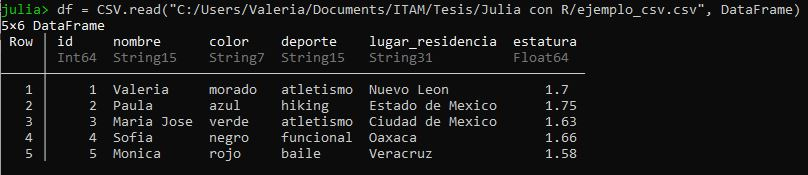
\includegraphics[scale=0.6]{Imagenes/insertar_df.JPG}
  \label{insertar_df}
\end{center}
\end{figure}

Los dataframes se pueden manejar de diferentes maneras. En este trabajo utilicé algunas de ellas, pero en caso de que tengas más dudas puedes consultar el manual oficial del paquete en \url{https://dataframes.juliadata.org/stable/}. 

\subsection{Regresiones}

\valinline{Buen link de ayuda \url{https://www.machinelearningplus.com/linear-regression-in-julia/}}

¿Cuál es el punto de tener una muestra de tamaño significativo si no sabemos analizarla? Una de las maravillas que nos regala la estadística es el uso de regresiones para intentar encontrar una explicación a los datos. Regresión es un método que permite a los investigadores resumir como predicciones o valores promedio de un resultado varían a través de variables individuales definidas como predictores. \citep{regression_other_stories} 

En pocas palabras, una regresión es una fórmula que intenta explicar como una variable depende otras. En Julia, esto se puede hacer con ayuda del paquete \texttt{GLM}, ya que facilita el cálculo de modelos lineales. Como todos los paquetes, primero hay que instalarlo usando los pasos en \ref{instalacion_paquete}. 

En este paquete la función principal se llama \texttt{glm}. En el manual oficial del paquete \cite{glm_manual} está descrita la manera en que se pueden generar modelos más avanzados. La función principal es \texttt{glm(formula, data, family, link)} donde 

\begin{itemize}
    \item \texttt{formula}: usa los nombres de las columnas del dataframe de datos para referirse a las variables predictoras
    
    \item \texttt{data}: el dataframe que contenga los predictores de las formula
    
    \item \texttt{family}: podemos elegir entre Bernoulli(), Binomial(), Gamma(), Normal(), Poisson() o NegativeBinomial() 
    
    \item \texttt{link}: se usa para especificar la función liga o \textit{link function}. La lista de posibles opciones está en el manual oficial de GLM. 
\end{itemize}


\subsubsection{Regresión lineal simple}
El modelo de regresión lineal más simple es el que tiene un solo predictor

\begin{equation*}
    \begin{aligned}
    y = a + bx + \epsilon
    \end{aligned}
\end{equation*}

Para ejemplificar este modelo de regresión use los datos de \citep{regression_other_stories}. Los datos fueron recabados por Douglas Hibbs con el objetivo de predecir las elecciones de Estados Unidos basándose solamente en el crecimiento económico. Los datos se ven de la siguiente manera: \val{Como le hago para incluir esto?}

\begin{figure}[H]
\begin{center}
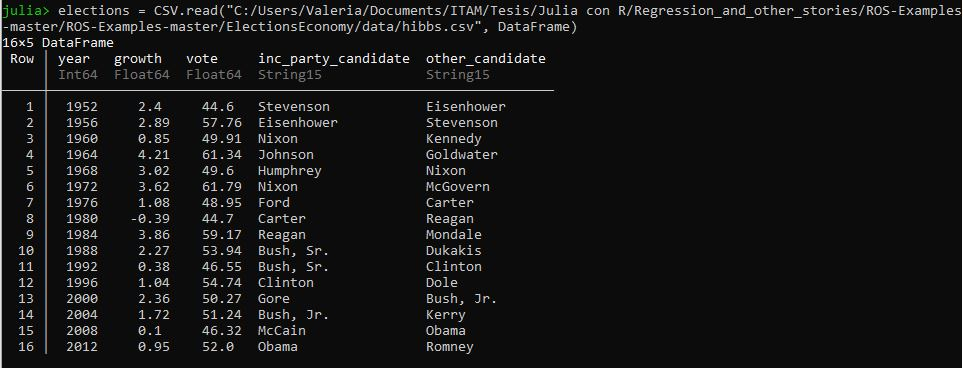
\includegraphics[scale=0.5]{Imagenes/elections_dataframe.JPG}
  \label{elections_dataframe}
\end{center}
\end{figure}

En este modelo busco que el voto sea resultado del crecimiento económico. El código para hacer esto en Julia es

\begin{minted}{julia}
	elections_lm = lm(@formula(vote ~ growth), elections)
\end{minted}

El resultado es una tabla con los coeficientes, la desviación estándar, el valor t, el valor p y el intervalo de confianza del $95 \% $ para los regresores. En este ejemplo, el resultado que da Julia es $y = 46.3 + 3.1x$ el cual coincide con los valores que da Gelman.

\subsubsection{Regresión lineal múltiple}

El caso general de la sección anterior se conoce como regresión lineal múltiple. La diferencia es que en este caso hay múltiples predictores que cumplen ciertos criterios. \cite{regression_other_stories} define este tipo de regresión como 

\begin{equation*}
    \begin{aligned}
    y_i = \beta_1 X_{i1} + \dots + \beta_k X_{ik} + \epsilon_i, \text{ para } i = 1, \dots, n
    \end{aligned}
\end{equation*}

donde los errores $\epsilon_i$ son independientes e idénticamente distribuidos de manera normal con media 0 y varianza $\sigma^2$. La representación matricial equivalente es 

\begin{equation} \label{eq_rlm}
    \begin{aligned}
        y_i = X_i \beta + \epsilon_i, \text{ para } i = 1, \dots, n
    \end{aligned}
\end{equation}

donde $X$ es una matriz de $n \times k$ con renglón $X_i$.

Para ejemplificar este tipo de modelo use un ejemplo que consta de dos predictores y la relación entre ellos. De nuevo utilicé los datos de \cite{regression_other_stories} que muestran la relación entre los resultados de exámenes de niños (\texttt{kid\_score}), el coeficiente intelectual IQ de sus madres (\texttt{mom\_iq}) y si sus madres terminaron o no la preparatoria (\texttt{mom\_hs}). 

Busco determinar si hay relación significativa entre la educación y el coeficiente de las madres con los resultados de exámenes de los niños. Por lo tanto, los predictores son las variables en relación con la madre mientras que la respuesta es el desempeño de los niños. El código en Julia se ve de la siguiente manera

\valinline{Como pongo el directorio de donde está mi base?}
\begin{minted}{julia}
    using DataFrames, GLM, CSV

    data_kid = CSV.read("C:/Users/Valeria/Documents/ITAM/Tesis/Julia con R/Regression_and_other_stories/ROS-Examples-master/ROS-Examples-master/KidIQ/data/kidiq.csv", DataFrame)

    fm = @formula(kid_score ~ mom_hs + mom_iq + mom_hs*mom_iq)

    kidscore_lm = lm(fm, data_kid)
\end{minted}

Lo cual da como resultado el modelo 

\begin{equation*}
    \begin{aligned}
        kid\_score = -11.48 + 51.26* mom\_hs + 0.97*mom\_iq \\
        -0.48*mom\_hs*mom\_iq + \epsilon
    \end{aligned}
\end{equation*}

Otro de los aspectos que hay que resaltar en este ejemplo es que para incluir la relación entre dos predictores basta usar un asterisco entre ellos al momento de definir la formula de la regresión. 

En el caso donde alguno de los regresores sea de tipo categórico la fórmula se mantiene igual pero hay que hacerle cambios a la base de datos en sí. Si Julia no reconoce estas columnas como categóricas entonces hay que cambiar su tipo en el dataframe. Abordo este problema más a fondo en el capítulo 8 \val{Checar al final que sí sea este capítulo}. Por otro lado, puedes intentar usar el paquete \texttt{CSVFiles} para leer los archivos ya que hace mejor trabajo identificando el tipo de variables. Sin embargo, este paquete todavía está en desarrollo por lo es más propenso a tener errores. 

\chapter{\textit{Polynomials}}

Polynomials es un paquete de Julia que proporciona arimética básica, integración, diferenciación, evaluación, raíces para polinomios univariados \cite{poly_manual}. Para instalar el paquete hay que seguir los comandos \ref{instalacion_paquete}. Esta sección va a explicar como ajustar un polinomio a un conjunto de datos. 

\section{El problema}
Supongamos que tenemos un conjunto de datos con solamente dos variables $x$ y $y$. Buscamos ajustarlos a un polinomio de grado $k$. Es decir, buscamos ajustar los datos al modelo

\begin{equation} \label{eq_polinomio}
    \begin{aligned}
    y = \sum_{j = 0}^{k} \beta_j x^j + \epsilon
    \end{aligned}
\end{equation}

El problema consiste en encontrar los mejores coeficientes que cumplan la ecuación anterior. Para hacerlo, el paquete Polynomials utiliza una implementación del método de Gauss-Newton para resolver un problema de mínimos cuadrados no lineal. \val{Ya sé que dice que es para problemas no lineales y el mío es un problema lineal pero es el único que funciona}


\section{Método Gauss-Newton}
\valinline{Supongo que lo tengo que explicar???}



\section{Ejemplo}
Para probar la función \texttt{fit} del paquete Polynomials elegí utilizar el conjunto de datos llamado \textit{Filip} del Laboratorio de Información Tecnológica perteneciente al Instituto Nacional de Estándares y Tecnología (NIST por sus siglas en inglés). Los datos y el resultado de la estimación de coeficientes están en \url{https://www.itl.nist.gov/div898/strd/lls/data/LINKS/DATA/Filip.dat}. 
\\
El código en Julia para obtener el resultado es el siguiente: 

\begin{minted}{julia}
    using Polynomials
    filip = CSV.read("filip_data.csv", DataFrame)
    coef_filip = CSV.read("coeficientes_filip.csv", DataFrame)
    x = filip.x
    y = filip.y
    as = coef_filip.coeficiente
    p = Polynomials.fit(x,y, 10)
\end{minted}

Los datos con las 82 observaciones en forma de pares ordenados es \texttt{filip\_data.csv}, mientras que los datos con los resultados de los coeficientes dados por el NIST es \texttt{coeficientes\_filip.csv}. Dichos documentos fueron obtenidos de la página mencionada anteriormente. 
\\
El resultado obtenido en Julia es \val{Lo voy a dejar asi aunque se ve pésimo, solo es para que se vean todos los coeficientes}

\begin{tcolorbox}
    \begin{verbatim}
    -1467.4896770751313 - 2772.179712060834x
    - 2316.3711834983233x^2 - 1127.973991485157x^3 -
    354.478249903365x^4 - 75.12420525407894x^5 -
    10.875318557918678x^6 - 1.0622150384213702x^7 -
    0.06701911888098762x^8 - 0.0024678109131484544x^9 -
    4.0296254716574806e-5x^10
    \end{verbatim}
\end{tcolorbox}

\valinline{OJO, no me da el error de la estimación, ni valor t ni nada}

Para comparar los resultados con las estimaciones reales de los coeficientes, uso el siguiente código de Julia:

\begin{minted}{julia}
    as = coef_filip.coeficiente
    q = Polynomial(as)
    maximum(abs(p(x) - q(x)) for x in range(0,1, length=1000))
\end{minted}

Es decir, creo un polinomio con las estimaciones de los coeficientes de NIST y después hago la diferencia en valor absoluto con la estimación que yo obtuve. El resultado es

\begin{tcolorbox}
    \begin{verbatim}
        0.0003723332774825394
    \end{verbatim}
\end{tcolorbox}

Por lo tanto, en la peor estimación de $\beta_i$, Julia acierta hasta 3 dígitos. 


\chapter{R}
Porque juntar Julia con R. Usar documentación oficial: https://cran.r-project.org/web/packages/JuliaCall/JuliaCall.pdf. También en esta sección incluir muchos ejemplos prácticos 

\section{Paquete JuliaCall}
Como instalarlo en R 

\subsection{install\_julia}

\subsection{julia\_setup}
De este no estoy segura, tengo que checar en las cosas de Rodrigo

\subsection{Núcleos y threads}

\subsection{JuliaObject}

\subsection{julia\_assign}

\subsection{julia\_eval}

\subsection{julia\_package}

\section{Ejemplo}
\chapter{Computadoras virtuales}

\section{Amazon}
Como hacer una computadora virtual en Amazon que me haga todo esto. El tutorial oficial de como instalarlo en Amazon está aquí: \url{https://d1.awsstatic.com/whitepapers/julia-on-sagemaker.pdf?did=wp_card&trk=wp_card}

\section{Docker}
También se podría usar Docker pero te quita espacio en tu computadora y puede crashear como la mía. Para Windows como que no está muy bonito el asunto pero al parecer para Linux sí. También podría ser opción idk 


%----------------------------------------------------------------------------------------
%	APÉNDICES
%----------------------------------------------------------------------------------------

\begin{appendix}

\chapter{Extras}
No se olviden cambiar toda la información. Los quiero un chingo

\end{appendix}

%----------------------------------------------------------------------------------------
%	BIBLIOGRAFÍA
%----------------------------------------------------------------------------------------

\bibliography{referencias}
\bibliographystyle{chicago}

\newpage
\thispagestyle{empty}
\begin{center}
\begin{minipage}{.6\linewidth}
\begin{center}
\vspace{3cm}
\begin{small}
\textit{\thetitle}, escrito por \theauthor , se terminó de imprimir de madrugada,\\ con mucha cafeína en las venas\\ y ojeras en la cara. %Le ponen el nombre del lugar donde la manden a imprimir, la ciudad y el año
\end{small}
\end{center}
\end{minipage}
\end{center}

% Si lo prefieren, avisen a su taller que esta página ya la incluyeron ustedes para que no les impriman las que ellos usan. Lo recomiendo ampliamente

%%%%%%%%%%%%%%%%%%%%%%%%%%%%%%%%%%%%%%%%%%%%%%%%%%%%%%%%%%%%%%%%%%%%%%%%%%%%%%%%%%%%%%%

\end{document}